\section{Regularization Experiments}

Another hyperparameter that may help improve generalization is
regularization. We introduce a new term in the computation of error, $\lambda C$
that measures the complexity of the model. Here, $\lambda$ is the
hyperparameter we tune (typically a small value) to adjust the
strength of the regularization. Altogether, we have a new measure of error

\begin{equation*}
	J = E + \lambda C
\end{equation*}

Here, $C$ can take various forms. Two well-known forms include $L_1$ and $L_2$
regularization.

$L_1$ regularization seeks to minimize $C = |W|$. Therefore,

\begin{equation*}
	\begin{aligned}
		\frac{\partial J}{\partial w_{ij}} & = \nabla E^{(n)}(w_{ij}) + \lambda
		\frac{\partial C}{\partial w_{ij}}                                      \\
		                                   & = \nabla E^{(n)}(w_{ij}) + \lambda
		\text{sign}  (w_{ij})                                                   \\
	\end{aligned}
	\label{eq:l1_l2}
\end{equation*}

where the matrix of ones $\mathbf{1} \in \mathbb{R}^{i \times j}$. On the other
hand, $L_2$ regularization seeks to minimize $C = \| W \|^2_2$.

\begin{equation*}
	\begin{aligned}
		\frac{\partial J}{\partial w_{ij}} & = \nabla E^{(n)}(w_{ij}) + \lambda
		\frac{\partial C}{\partial w_{ij}}                                        \\
		                                   & = \nabla E^{(n)}(w_{ij}) + 2 \lambda
		w_{ij}                                                                    \\
	\end{aligned}
\end{equation*}

\subsection{Experiments}
In our previous experiments with momentum and early stopping, we achieved a test
accuracy of $96.62\%$ within 7 epochs. We will run our regularization
experiments with approximately $10\%$ more epochs (8 total epochs). We achieve
the following results

\begin{figure}[H]
	\begin{subfigure}{0.5\textwidth}
		\centering
		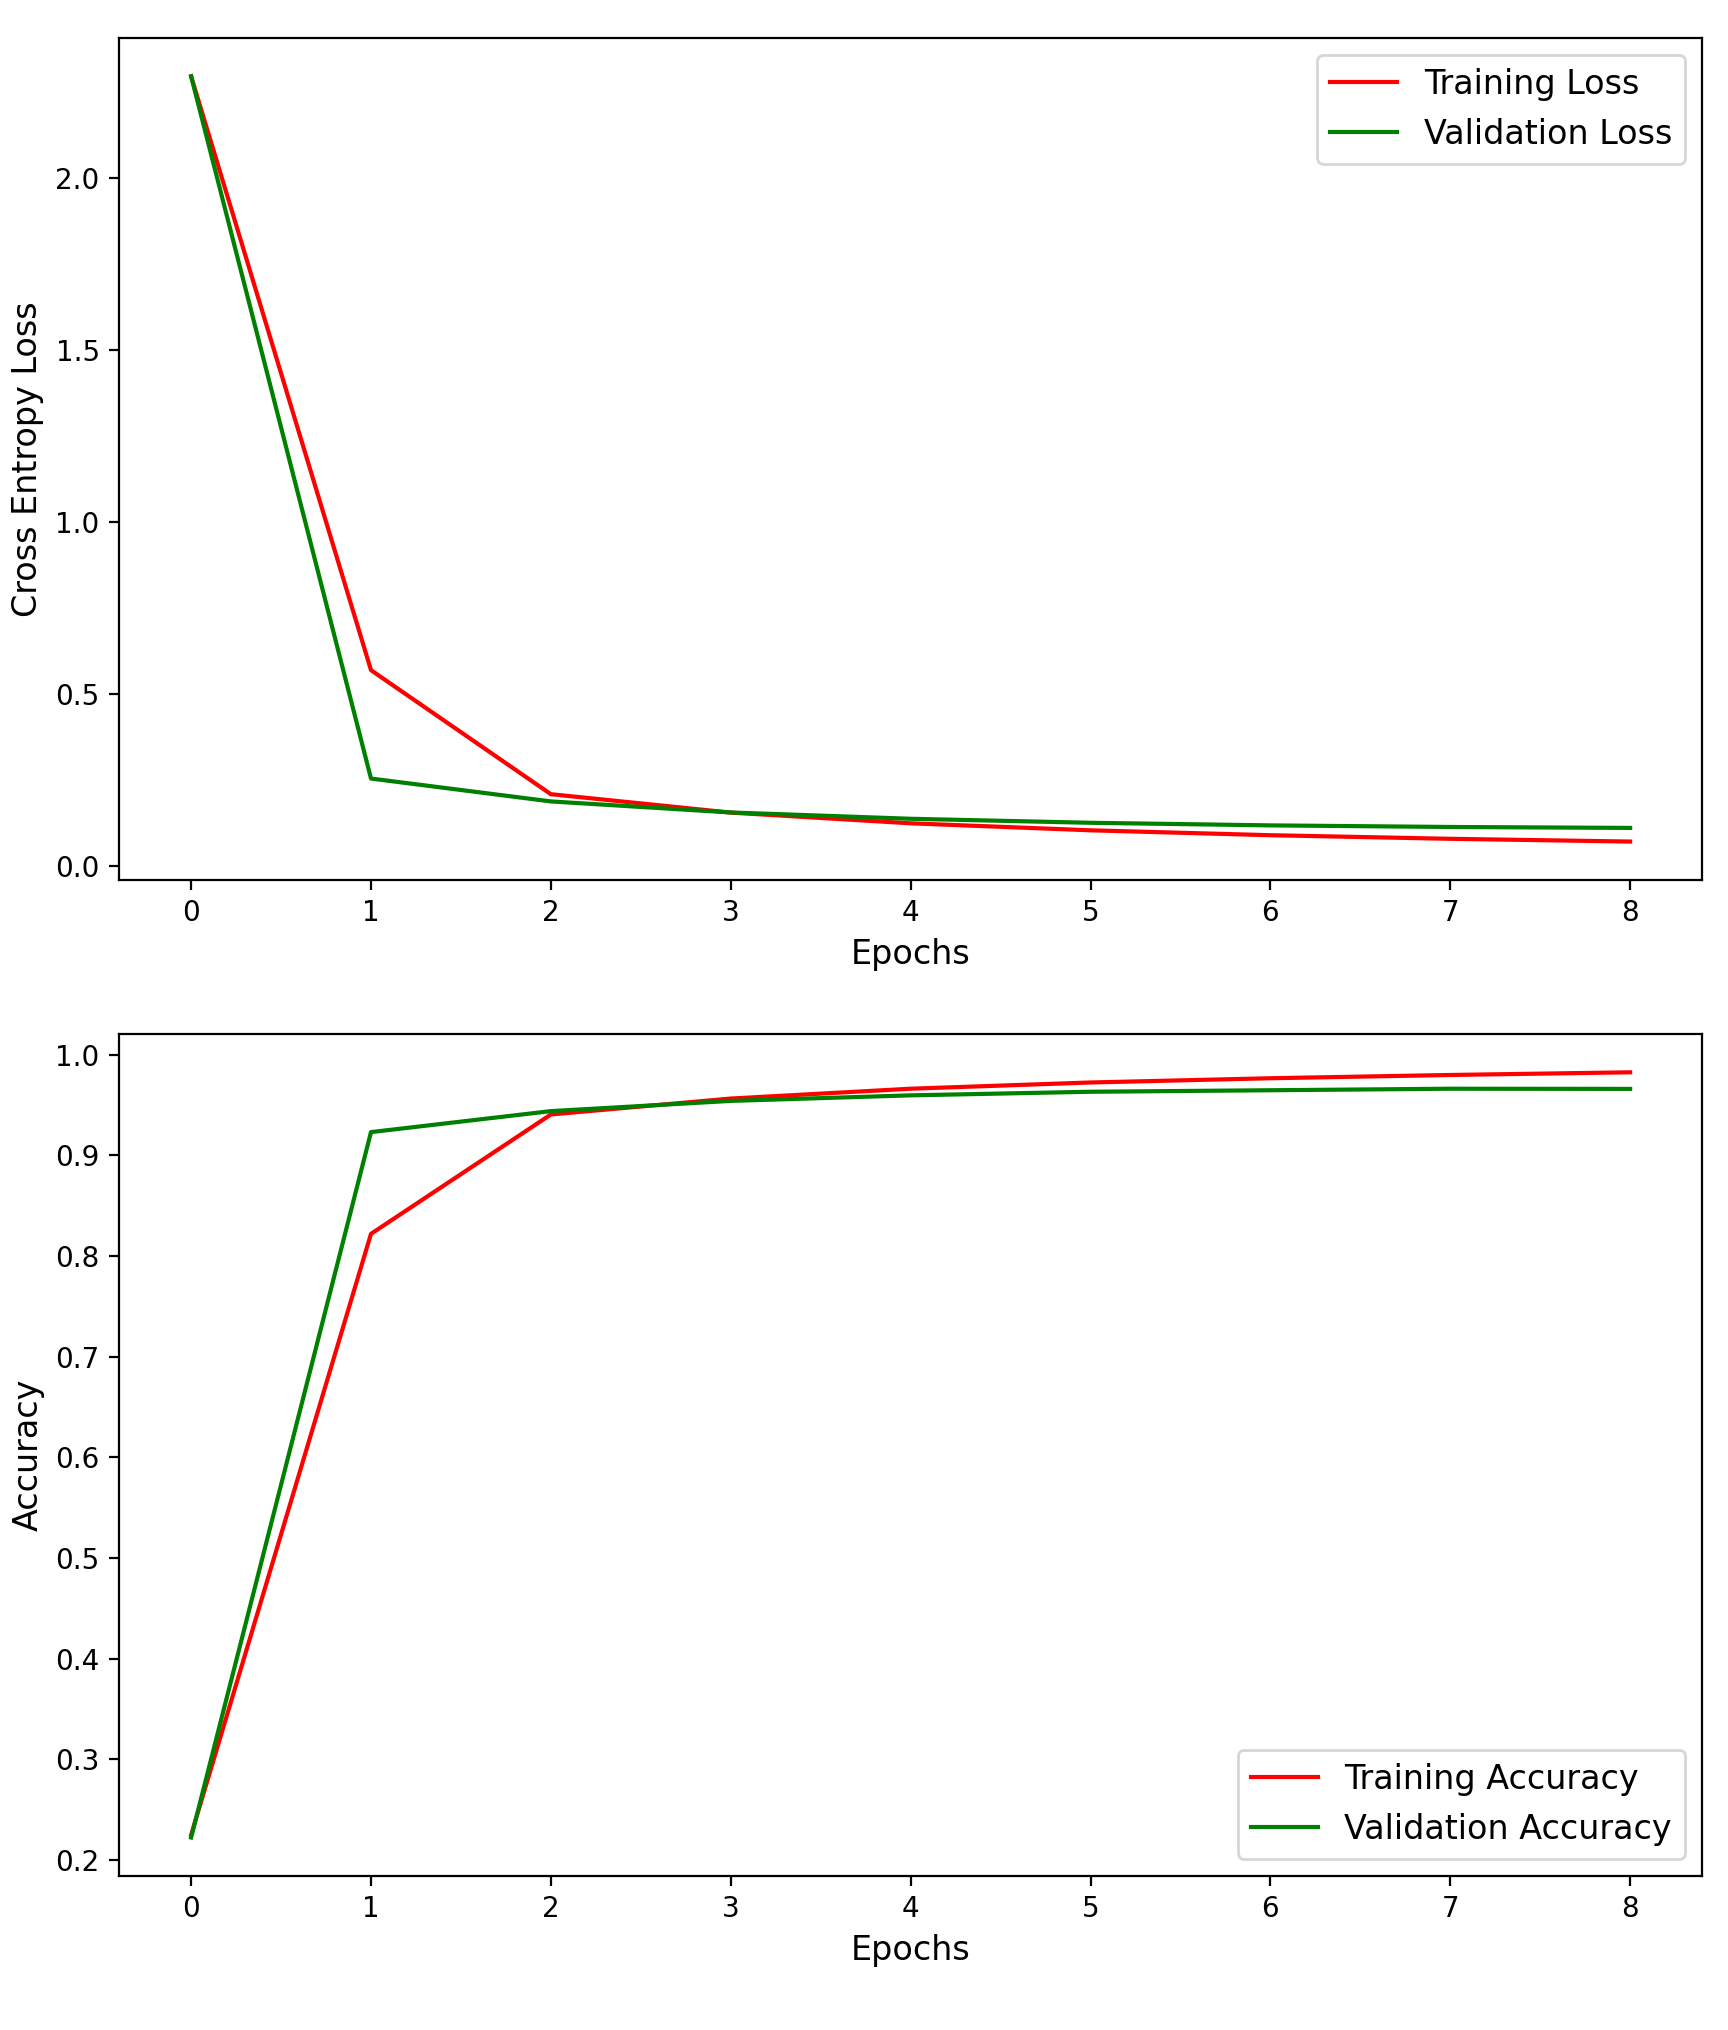
\includegraphics[width=1.0\textwidth]{./images/l1_e2.png}
		\caption{$L_1$ Regularization with $\lambda = 1e^{-2}$}
		\label{fig:l1_1e2}
	\end{subfigure}
	\begin{subfigure}{0.5\textwidth}
		\centering
		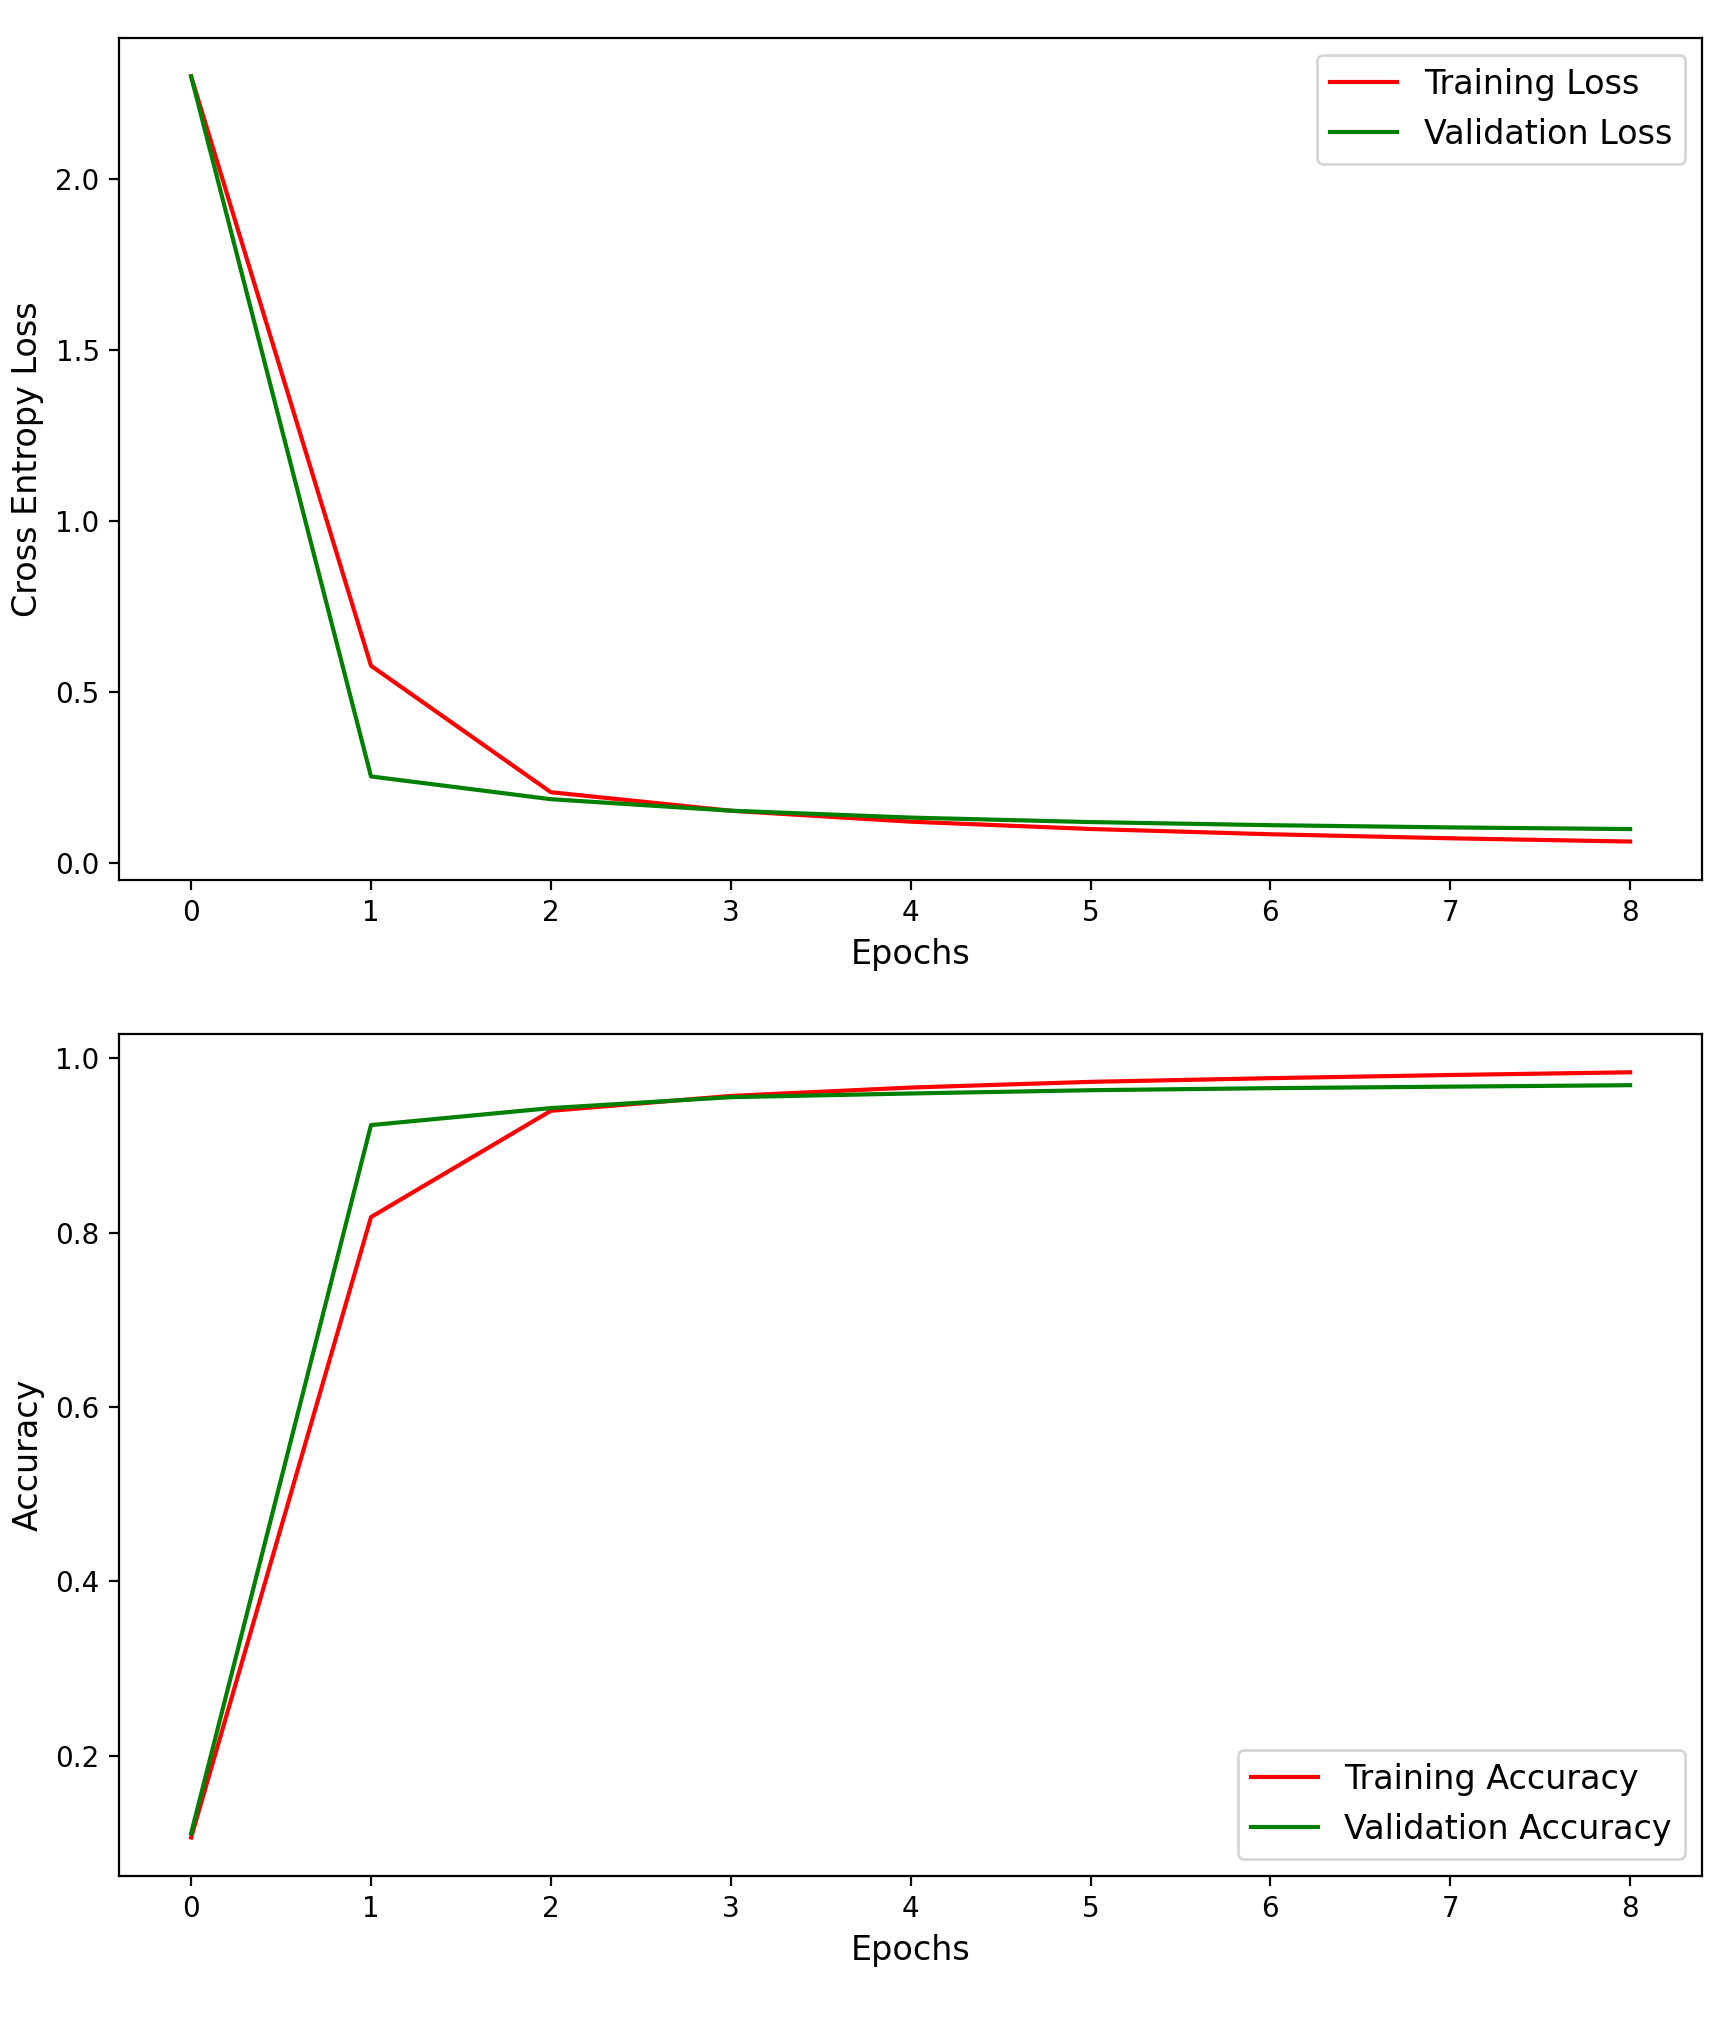
\includegraphics[width=1.0\textwidth]{./images/l1_e4.png}
		\caption{$L_1$ Regularization with $\lambda = 1e^{-4}$}
		\label{fig:l1_1e4}
	\end{subfigure}

	\begin{subfigure}{0.5\textwidth}
		\centering
		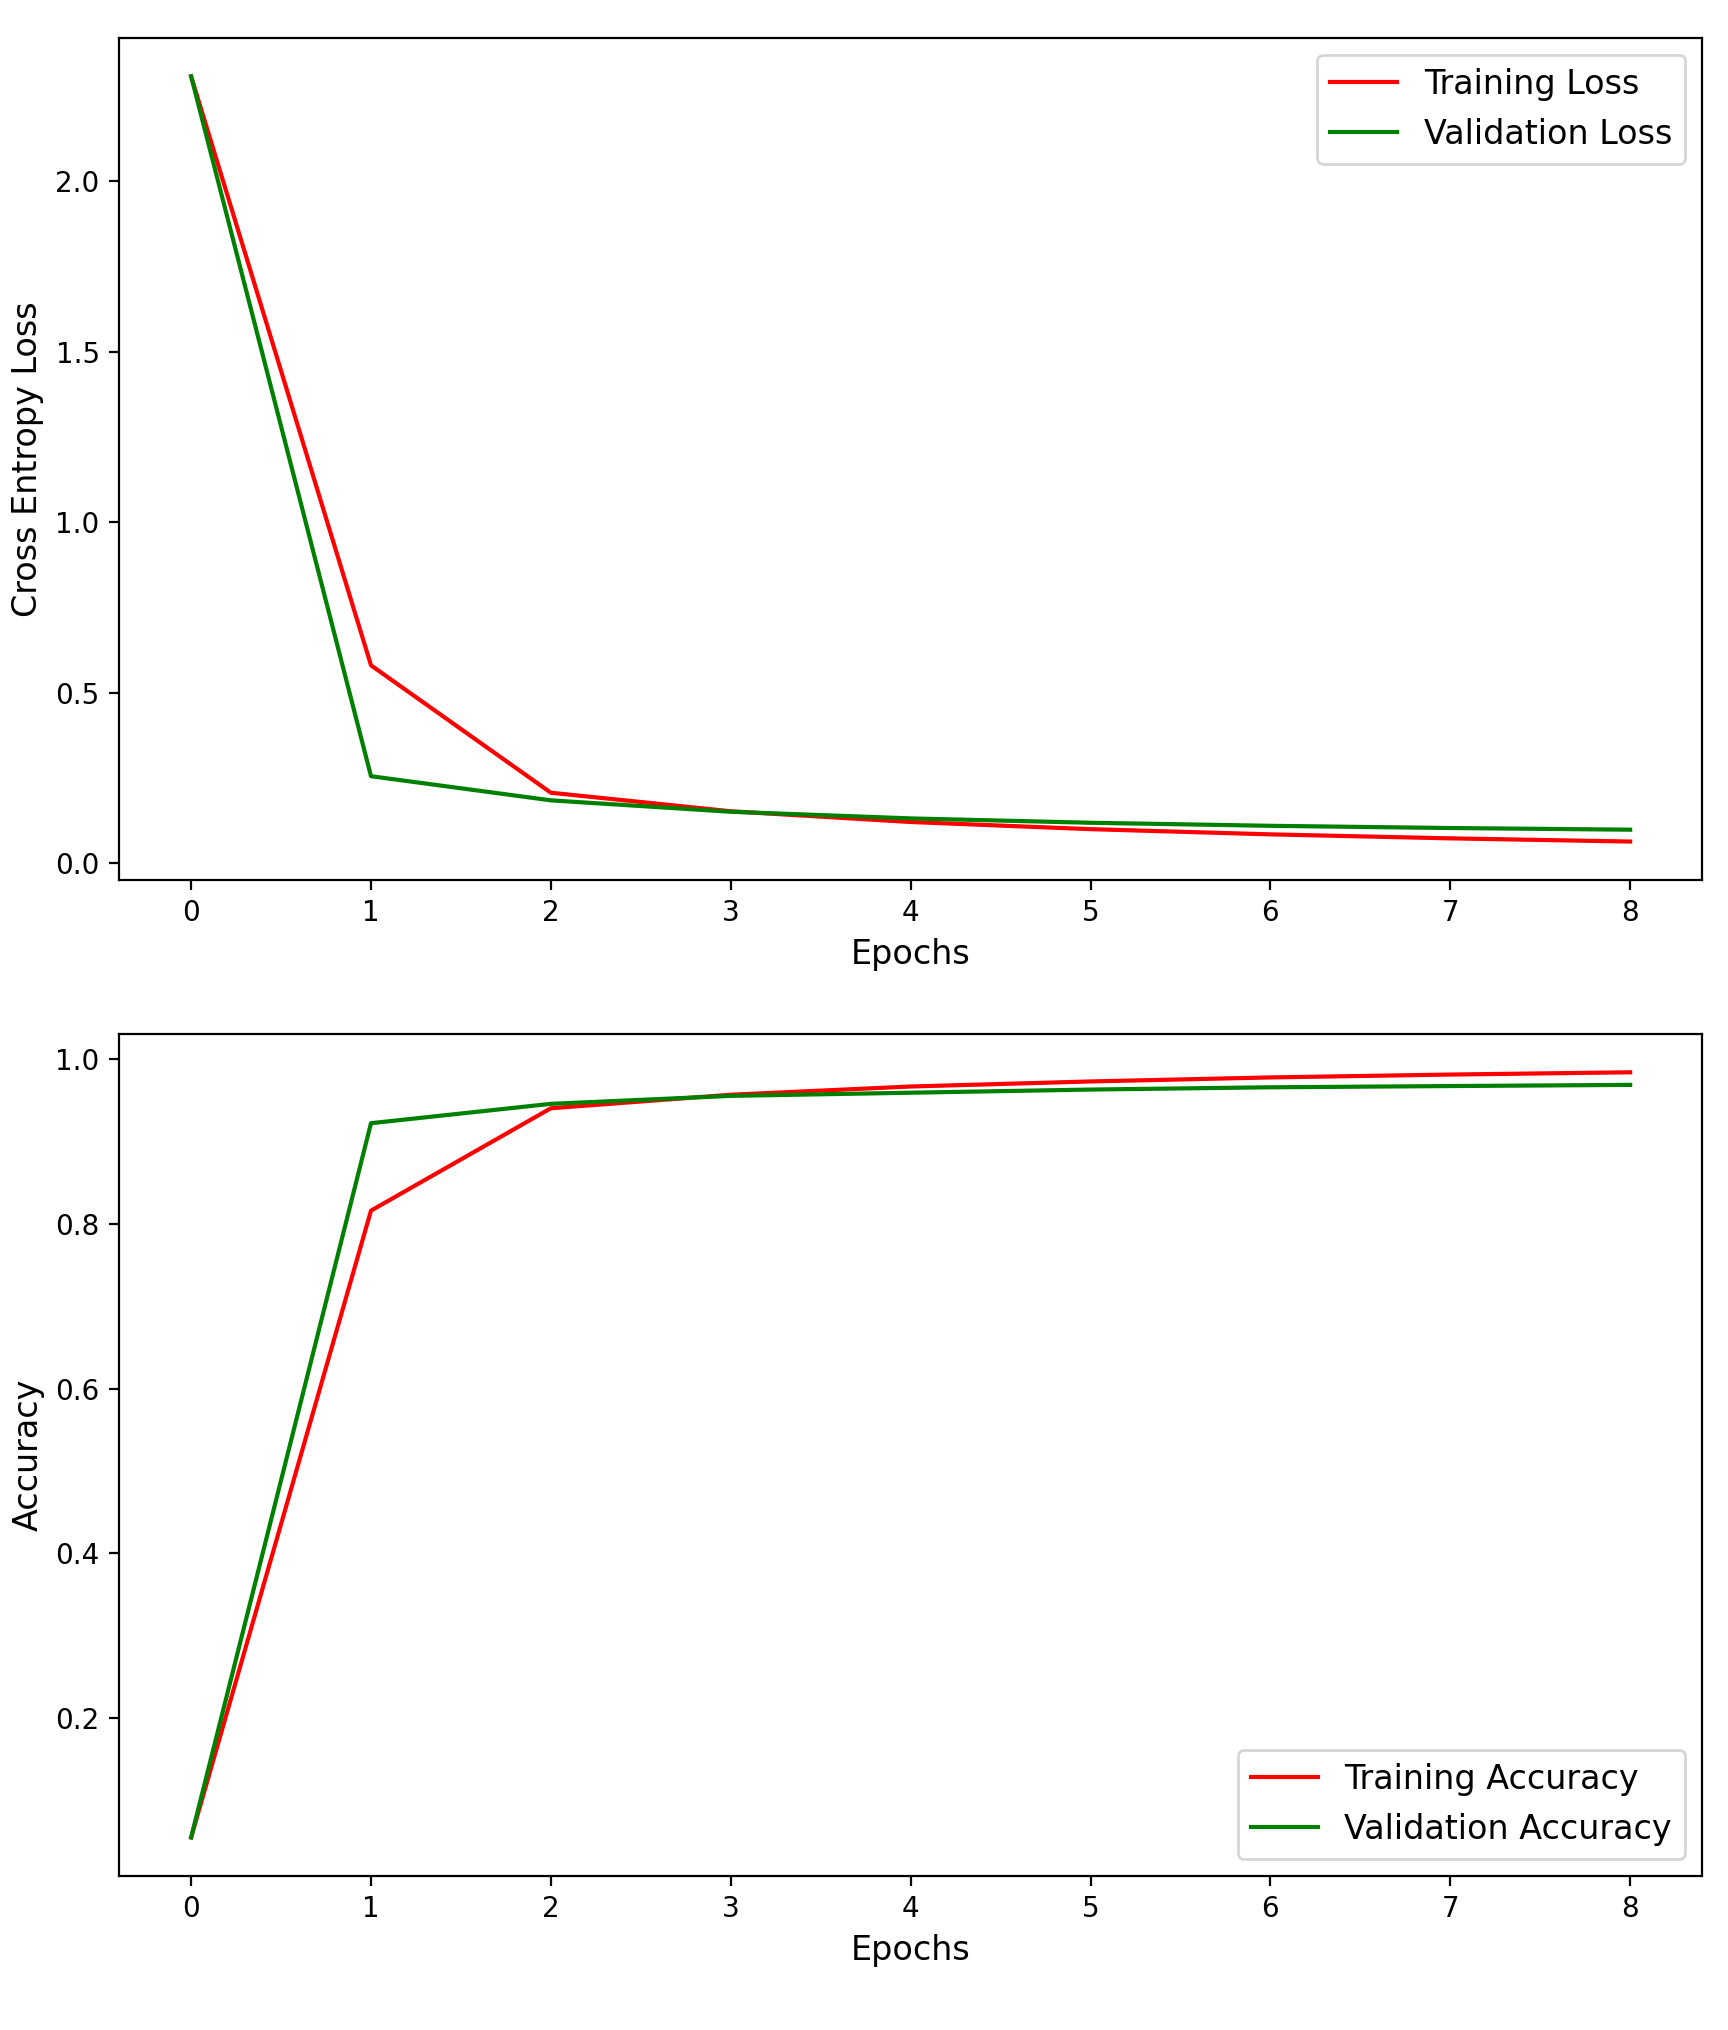
\includegraphics[width=1.0\textwidth]{./images/l2_e2.png}
		\caption{$L_2$ Regularization with $\lambda = 1e^{-2}$}
		\label{fig:l2_1e2}
	\end{subfigure}
	\begin{subfigure}{0.5\textwidth}
		\centering
		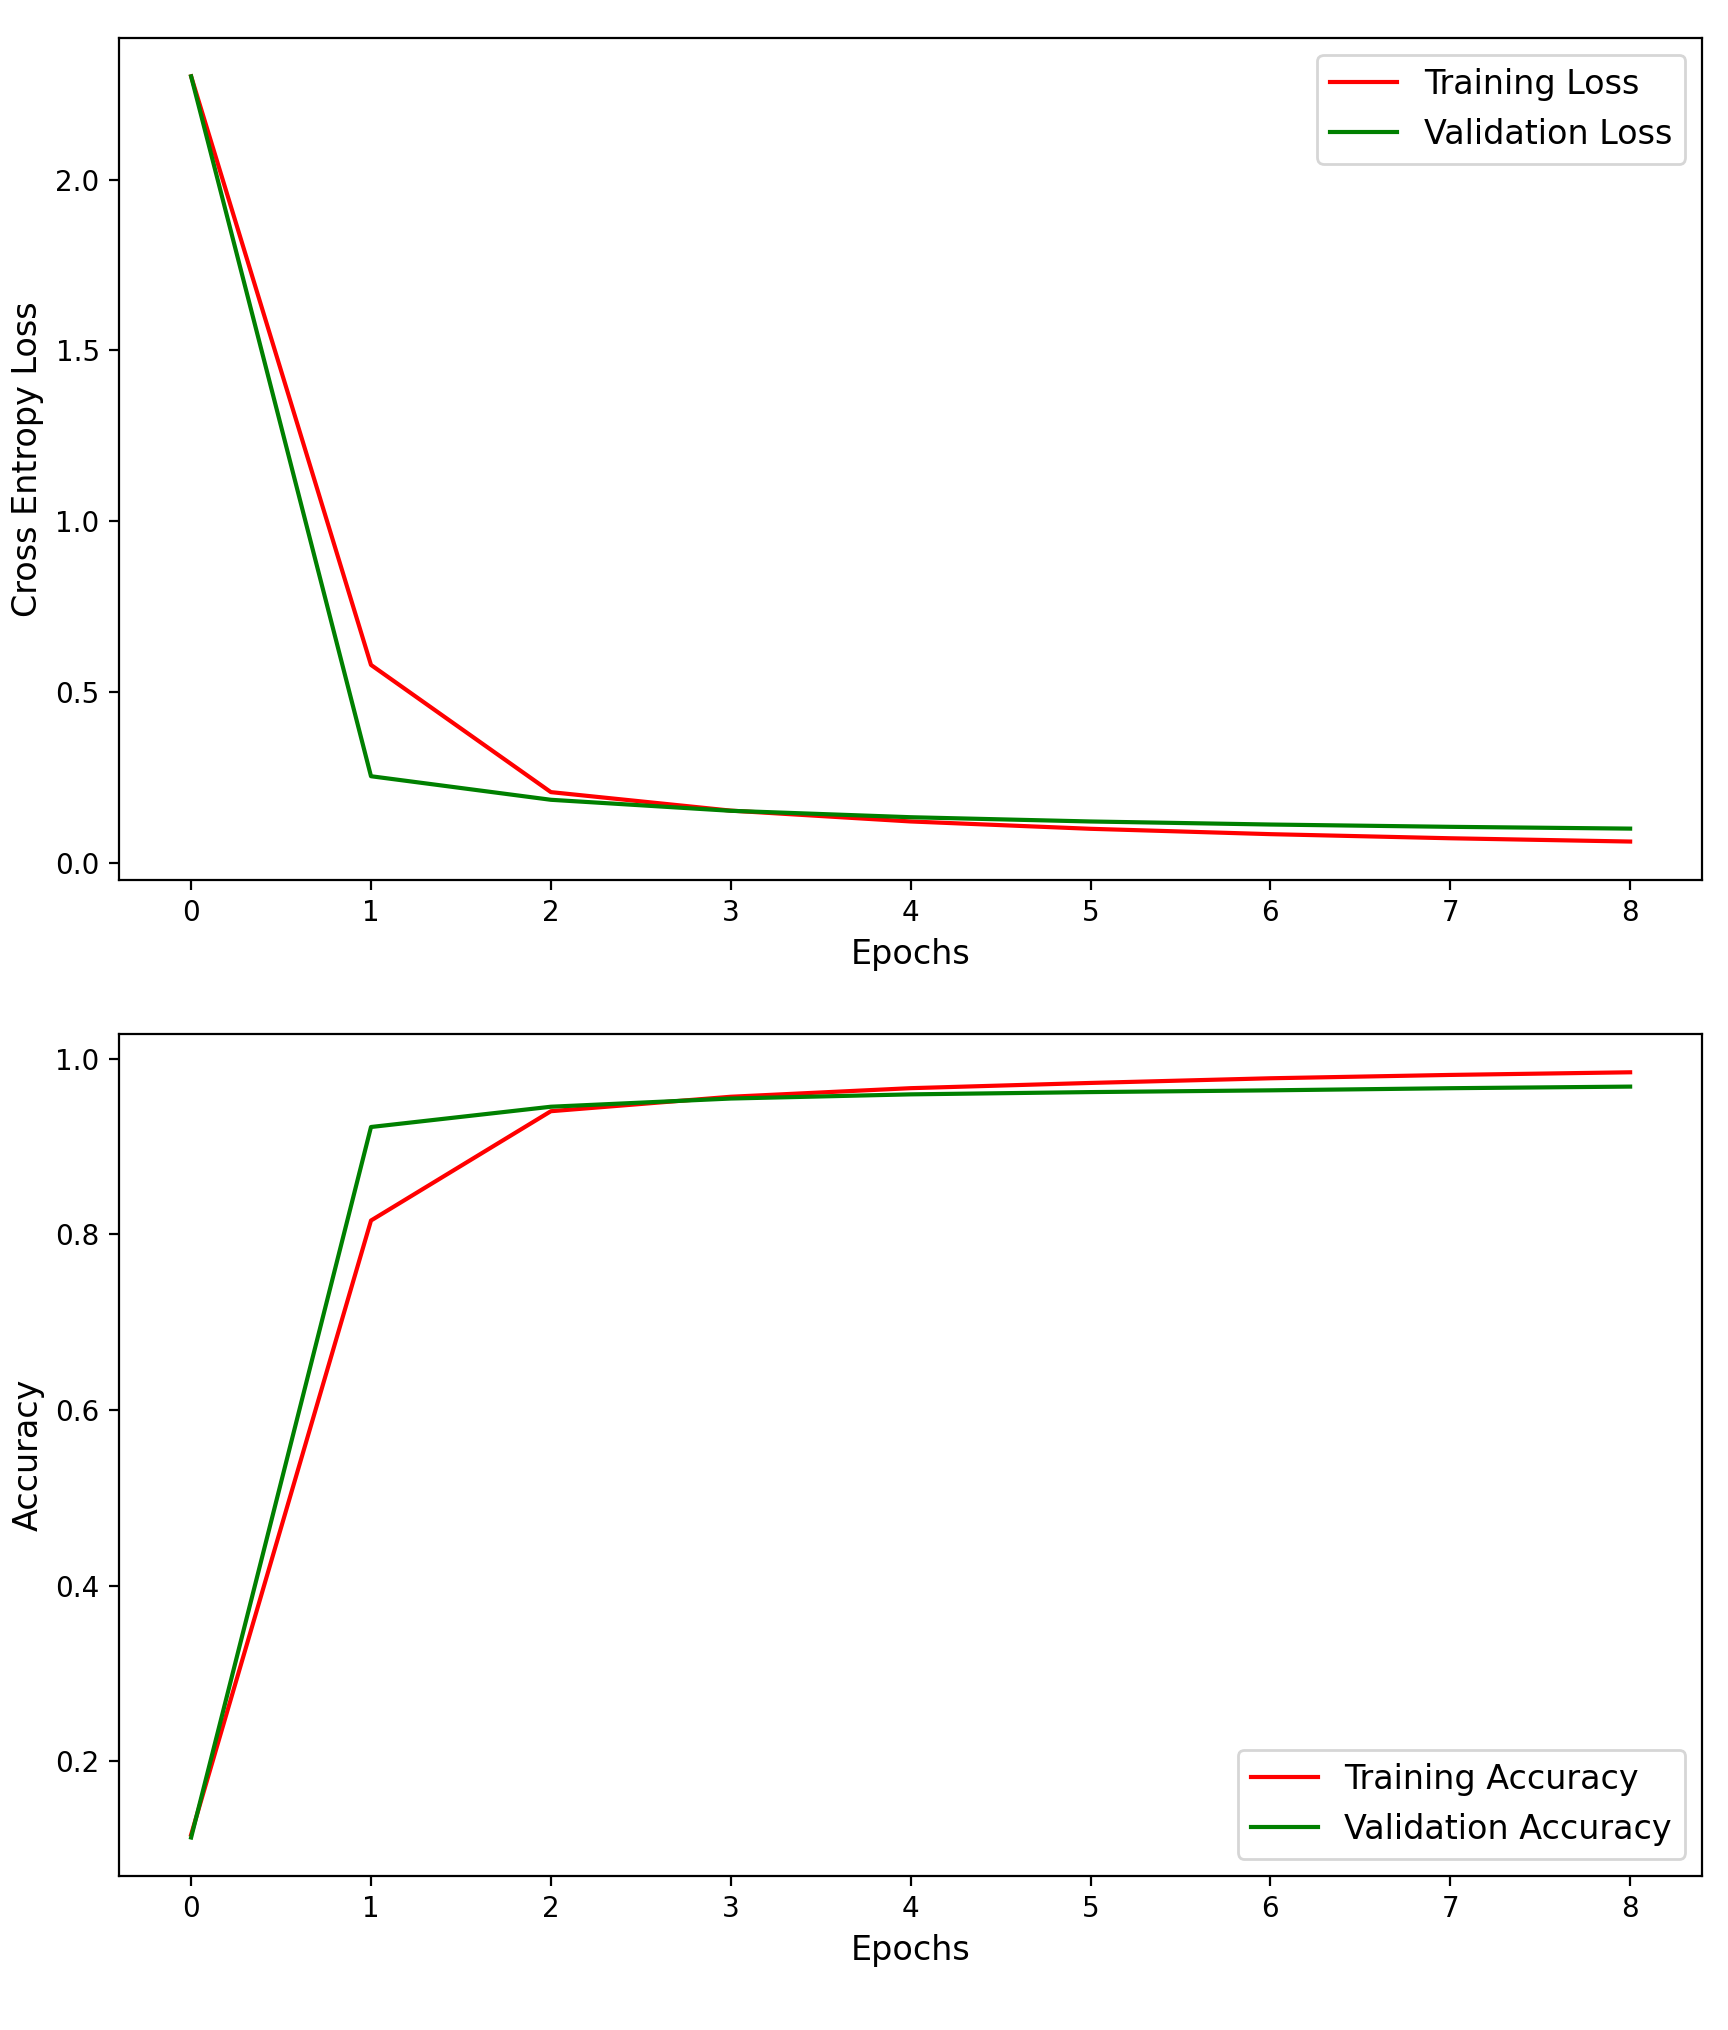
\includegraphics[width=1.0\textwidth]{./images/l2_e4.png}
		\caption{$L_2$ Regularization with $\lambda = 1e^{-4}$}
		\label{fig:l2_1e4}
	\end{subfigure}
\end{figure}

\subsection{Observations}
Overall, we see a trade-off between the speed of convergence, and the accuracy of the model. Here, speed of convergence refers to number of epochs it takes to reach a patience limit (number of epochs where the validation error increases). In general, as the $\lambda$ penalization term increases in both $L_1$ and $L_2$ regularization, the model takes longer to converge but reaches greater accuracy. As $\lambda$ decreases, the model converges more quickly but at the expense of some accuracy. In our experiments, a value of $\lambda = 0.0001$ with $L_2$ regularization achieves the greatest accuracy.

This trade-off is related to how important minimizing the size of the weights is. In the case where $\lambda$ is large, we spend more time searching for a minima given a set of small weights. In the case where $\lambda$ is small, we spend less time looking for a minima with small weights and pay more attention the gradient instead.

$L_1$ and $L_2$ ~\ref{eq:l1_l2} differ in that $L_1$ changes by some constant regardless of how large or small the weights are, while $L_2$ changes by a factor of the magnitude of the weights. As a result, it is harder for $L_1$ regularization to converge, because there is no difference in the $L_1$ penalization regardless of how large the weights are. However, $L_2$ regularization changes proportionally to the weights, resulting in the heavy penalization of very large weights while less penalization of smaller weights.
